\chapter{\iftoggle{german}{Einführung}{Introduction}}\label{ch:introduction}

As the Deep Learning field goes deeper and broader, data on large scales has become an essential requirement.
The performance of computer vision based on deep learning models heavily depends on the consistency of labeled images.
In practice, collecting data manually is time-consuming, expensive, and needs much effort.
As a solution, we can train models on a synthetic dataset and deploy the models to real-world problems.
Unfortunately, with supervised learning, the model does not generalize when the distributions of the dataset diverge.
Hence, a model trained on a synthetic dataset may not perform consistently with real-world data.

Synthetic data can be defined as data created artificially using computer simulations or algorithms and not from real-world events.
These data can be created in abundance and hence are frontrunners for Deep Learning training.
Synthetic approaches are also means of getting data that might be difficult to collect and annotate in the real world.
Furthermore, companies have realized that synthetic data are necessary not just for the task that is inconvenient to annotate,
but also for improving the performance of existing models.
In a research article published by Gartner\footnote{\label{gartnerreport}https://www.gartner.com/en/documents/4002912}, they claim that by 2030, synthetic datasets will overshadow a real dataset in all domains.
The progression of synthetic data generation is predicted to be as shown in \autoref{fig:Gartner research on synthetic dataset}.

\begin{figure}
    \centering
    \includegraphics[width=1.0\textwidth]{/Users/apple/OVGU/Thesis/code/3dReconstruction/report/images/intro/Gartner-chart_3}
    \caption[Evolution of Synthetic Datasets Over Time.]{A graph showing how synthetic dataset will evolve overtime. The research graph shows that synthetic dataset will overshadow the existing real dataset\textsuperscript{\ref{gartnerreport}}.
    Source: Research article from Gartner on "Synthetic Data Is the Future of AI"\textsuperscript{\ref{gartnerreport}}}
    \label{fig:Gartner research on synthetic dataset}
\end{figure}

Deep Learning has made leaps and bounds in solving 2D-image tasks like classification, segmentation, object detection, etc.
It has now entered the realm of Three-Dimension.
An image is a 3D objects projects onto a 2D surface.
While doing so, some data from the higher dimension is being lost in the lower dimension.
This inverse ability to reconstruct 3D objects from 2D images has a wide-scale application in computer vision and robotics.
Tasks like human body shapes and face reconstructions~\cite{deng2019accurate,Guo20193DFace,Afzal2020,Richardson2016,Richardson2017LearningDF},
3D-Scene reconstructions~\cite{Denninger20203DSR,Song2017SemanticSC,Li2019,Shin20193DSR}, generic object mesh reconstruction with textures are some of the advancements we had over recent years.
Here comes the challenge;3D data is not easy to collect.
3D data is not just limited but also noisy and expensive to collect.
The results of models depend on the consistency of the labeled data.
In this thesis, we discuss how game engines can contribute to generating quality-labeled datasets for 3D reconstruction tasks.

Deep Learning has made leaps and bounds in solving 2D-image tasks like classification, segmentation, object detection, and many more.
It has now entered the realm of Three-Dimension.
An image is a 3D objects projects onto a 2D surface.
While doing so, some data from the higher dimension is lost in, the lower dimension.
This inverse ability to reconstruct 3D objects from 2D images has wide applications in computer vision and robotics.
Tasks like human body shapes and face reconstructions~\cite{deng2019accurate,Guo20193DFace,Afzal2020,Richardson2016,Richardson2017LearningDF},
3D-Scene reconstructions~\cite{Denninger20203DSR,Song2017SemanticSC,Li2019,Shin20193DSR},
generic object mesh reconstruction with textures are some of the advancements we had over recent years.
Here comes the challenge;3D data is not easy to collect.
3D data is not just limited but also noisy and expensive to collect.

\section{Domain Adaptation vs. Domain Randomization} \label{sec:da vs dr}

As mentioned earlier, the success of Convolutional Neural Networks depends highly on the training data.
As it so happens, not every task will have abundant data to train.
One solution for this problem is using a pre-trained network of similar problems and using transfer learning.
The pre-trained network is then trained over with the limited data available for the problem at hand.
In this case, some layers get overwritten by fine-tuning the features learned from the larger dataset using a small annotated dataset of different domains.
Domain adaptation is a field of study in machine learning where training data distribution differs from testing or target distribution.
One shallow approach is, as mentioned above,
re-weighting the network with testing data to adapt to the problem domain~\cite{Li2017PredictionRF}.
``Deep domain adaptation methods leverage deep networks to learn more transferable representations by embedding domain adaptation in the pipeline of
deep learning"~\cite{Wang2018}.
For this thesis, domain adaptation is relevant as the synthetic dataset might not represent the real or target domain, leading to a drop in performance.

Domain randomization, on the other hand, is improving data quality such that the training domain includes that the target domain distribution.
The `reality gap'~\cite{tobin2017domain} gets negated with this approach between simulated environment and natural images.
This is achievable by randomizing the rendering of objects in the synthetic data.
The key concept here is that the real-world distribution will appear to be just a variation in the dataset by rendering objects with significant variance.
Textures, brightness, shadows, camera settings, and object pose are some of the features that can be randomized.
In \autoref{ch:concept} we will discuss domain randomization.


\section{Volumetric Representations of 3D Shapes} \label{sec:Volumetric representation}
The universal representation of images in computer graphics is via pixels.
However, unlike 2D, 3D data can be represented in various formats like voxels, mesh and point clouds.
\autoref{fig:3d representation} presents the representation of these three formats.
Each of the representations has its own sets of advantages and disadvantages.
Voxels, which is short for Volumetric Pixels, is a 3D grid of pixels of constant size.
As indicated in~\cite{li2016fpnn}, the main advantage of voxels is that Convolution Neural Networks can be easily applied to 3-Dimensions as in 2-Dimensions.
Since most of the 3D geometry is surface-based, it can be wasteful and computationally expensive.
Mesh is composed of vertices, edges, and faces in 3D space that indicates the formation of 3D objects.
This form of representation is far more compact at a granular level, depending on the resolution.
On the other hand, point clouds are collections of 3D points with (x,y,z) coordinates on the surface of the object.
The collection of points determines detailing the 3D object representation.
In both these cases, \gls{cnn} is not directly applicable which is a direct disadvantage.
However, since mesh and point clouds are surface-based, the memory consumption is less than voxels and thereby lesser computation time, which is their advantage over voxels.
In this thesis, we opt for voxel-based models as the focus is on the performance of synthetic data rather than the model or the 3D representation itself.

\begin{figure}
    \centering
    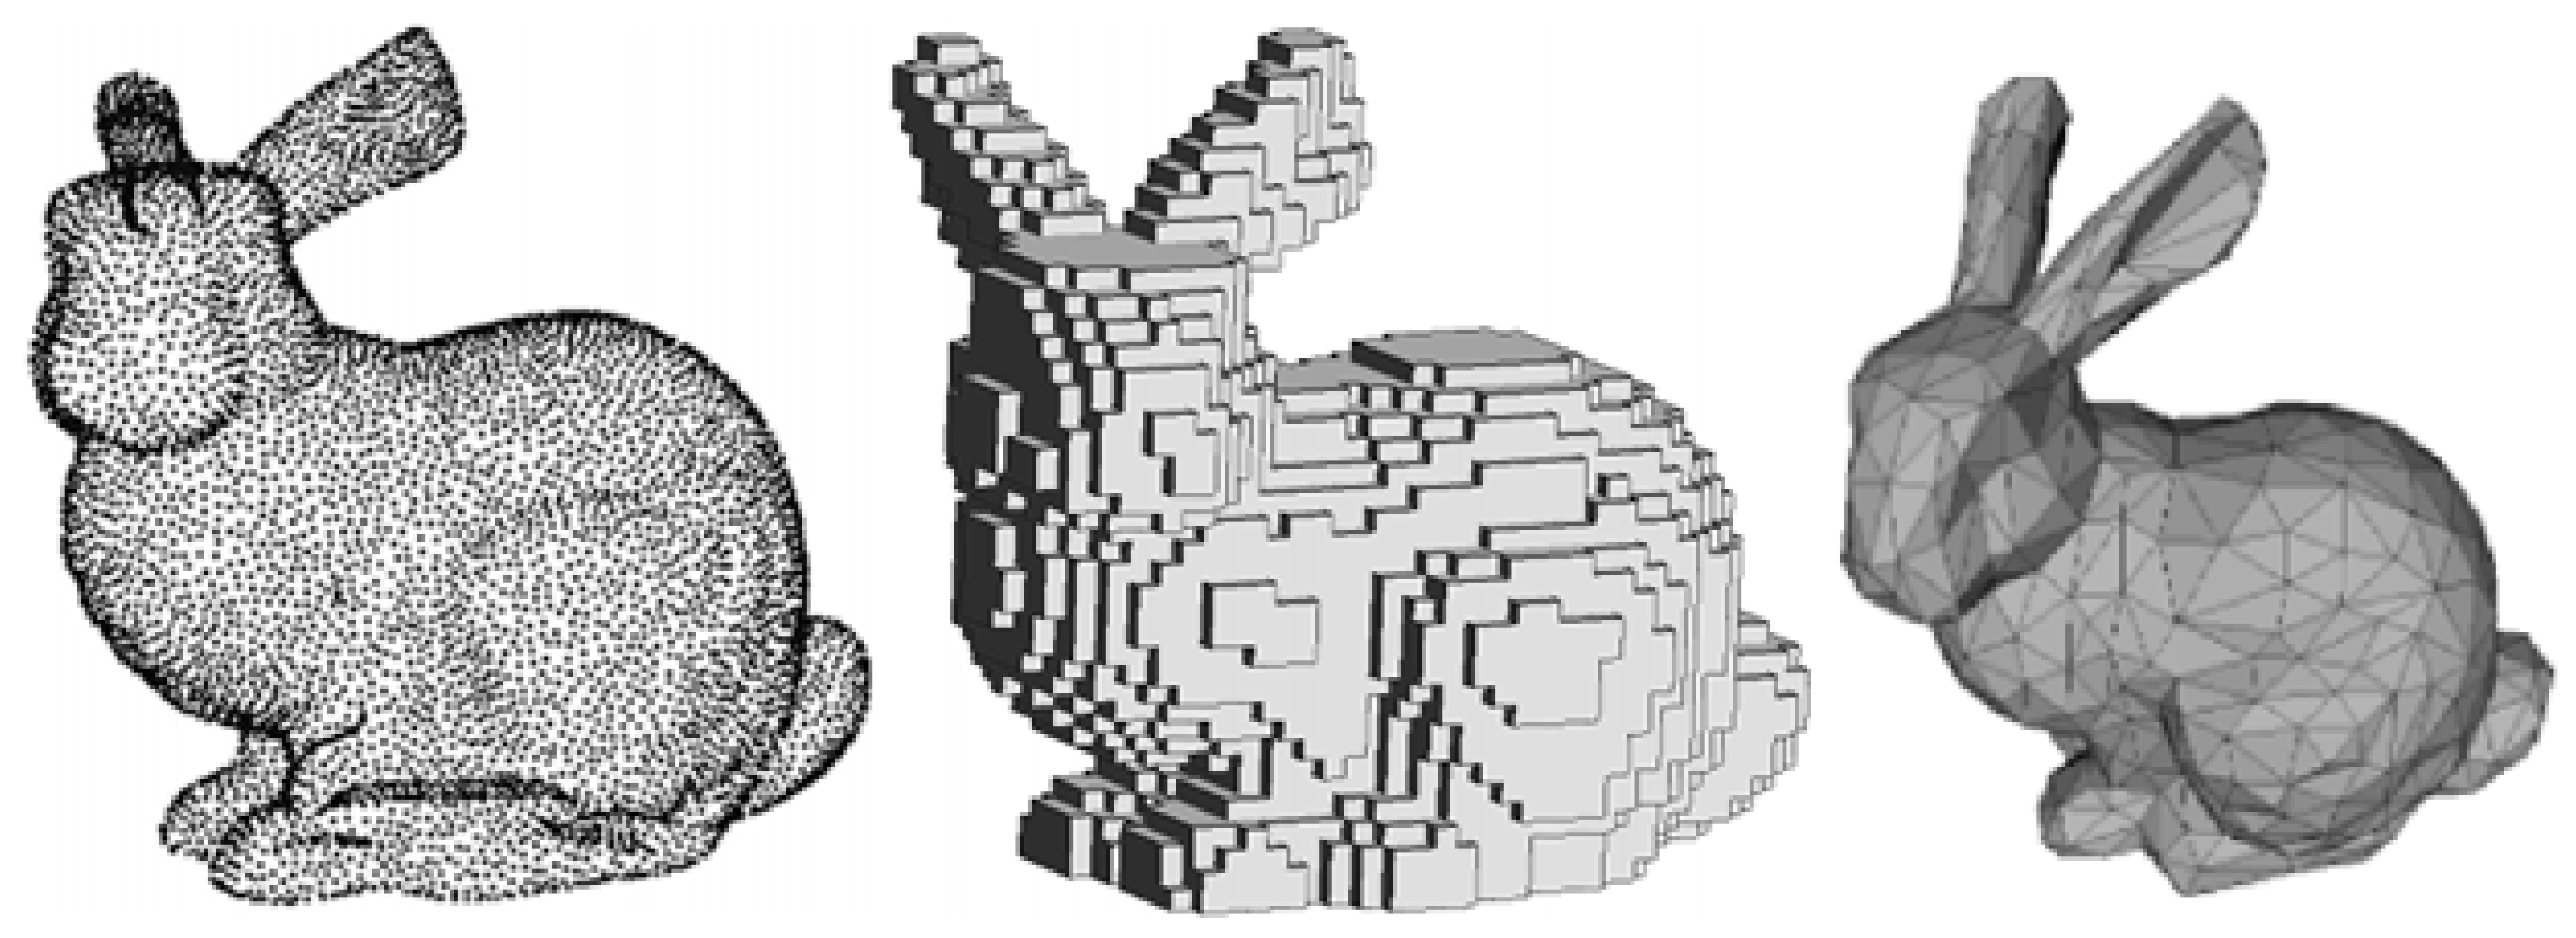
\includegraphics[width=1.0\textwidth]{/Users/apple/OVGU/Thesis/code/3dReconstruction/report/images/intro/3drepresentation}
    \caption[Types of 3D Representations]{3D representation of Standford bunny model.(left to right) Point cloud, voxel and mesh~\cite{Hoang2019ADL}
    \label{fig:3d representation}}
\end{figure}

\section{GameEngines}\label{sec:gameengines}
~\cite{Ee2005} defines a \emph{Game engine} as  “A series of modules and interfaces that allow a development team to focus on product gameplay content,
rather than technical content” Gold [2004].
In layman’s terms, game engines are software used for the development of games.
Unreal Engine, Unity, GameMaker, Amazon Lumberyard, and CryEngine are popular game engines in modern times.
Over time, the graphics in each game engine have improved to an extent where visually, we cannot differentiate between reality and graphics.
These use object-oriented techniques, which help in modularity.
Also, they are GUI-oriented and hence are user-friendly and accessible even to a novice programmer.
The critical component in game engines that we will be focusing on is the `Rendering engine’.
3D-Rendering is the means of converting 3D data into 2D images.
Rendering can either be real-time or offline/pre-rendering.
Game engines aim to make photorealism at the highest level with the least possible rendering time.


\section{Motivation}\label{sec:Background and motivation}

3D reconstruction is of great significance to understand a scene and to cross the 2D realm.
However, the task is not trivial, considering the input is still a Two-dimensional RGB image.
It is even more challenging since obtaining new data is expensive and time-consuming.
The 3D reconstruction field has datasets like ShapeNet~\cite{shapenet2015}, 3D-Front~\cite{Fu20203DFRONT3F}.
Nevertheless, there are no corresponding real images to check if the model will work in real-world scenarios.
Also, searching for real-world examples or creating a set-up scene and then labeling the images manually can lead to human mistakes resulting in wrong labels.
A solution to this problem is automating the task of generating synthetic data which can produce pixel-perfect annotations.
Automation can solve the human-in-the-loop problem, and while time gets saved, it facilitates the generation of a large quantity of data.
However, quantity should not be the only focus while creating the data;
we should also give priority to the quality of the data.
Game engines have come a long way from just supporting 2D to supporting games with photorealistic rendering.
Even though game engines have grown to be successful, few tools use them as the base framework.
As 3D models are available, we can import these models into the game engine and create an ersatz environment to generate a photorealistic dataset.
Further, we can check if these photorealistic synthetic data are useful for 3D reconstruction tasks.

\section{Goal of this Thesis}\label{sec:goal}

We will answer the following research questions:
\begin{enumerate}
    \item Are game engines a reliable medium for creating a photorealistic synthetic dataset?

    The photorealism of the images will be evaluated with a survey to compare images from the real dataset and generate datasets, and other proclaimed natural-looking datasets.

    \item Can Ersatz environment from a game engine like Unity replace real-world data for training in 3D reconstruction tasks?

    Using the dataset created with the Unity game engine, a single-view image to 3D reconstruction of furniture will be trained and tested on a real image dataset.

    \item Can we improve the performance of a model using a blend of real and synthetic datasets?
    To what extent does the performance enhance when the synthetic dataset is more than ten times of a real dataset?

    We use the dataset created using the Unity game engine to train a single-view image to 3D reconstruction of furniture and further fine-tune it with the real dataset to know if the performance is enhanced.
    Further an ablation study on chair dataset to check the effects domain randomization parameters.
    This experiment will also answer whether augmenting images with domain randomization with real data during training improves the performance?

\end{enumerate}

\section{Contributions of this Thesis}\label{sec:contributions}
In answering the research questions formulated in \autoref{sec:goal}, this thesis contributes the following:

\begin{itemize}
    \item A Unity-based framework to create a synthetic dataset with domain randomization.
    The tool supports both automated and manual image creation.
    \item A survey of photorealism to check whether Game engines produce quality synthetic datasets comparable with other proclaimed benchmarked photorealistic indoor datasets
    \item Provide a new dataset related to 3D reconstruction tasks or Synthetic to real domain adaptation tasks.
    The dataset includes G-buffers like RGB, normals, depth maps, and semantic segmentation images.
    \item Provide a focused synthetic chair dataset created with different parameters of domain randomization.
    A case study was conducted to check the influence of each component of domain randomization.
    \item A case study to understand the impact of mixed training.
    Synthetic and real image datasets are mixed in different ratios in each mini-batch to check the performance of the 3D reconstruction task.
    \item Fine-tuning models trained on a synthetic dataset with a small real dataset.
\end{itemize}


\section{Structure of this Thesis}\label{sec:Structure of thesis}

The rest of this thesis is structured as follows:

\begin{itemize}
    \item In \autoref{ch:related_work}, we visit some related work on synthetic data generation and benchmark 3D reconstruction networks.
    \item \autoref{ch:concept} deals with concepts and design choices.
    We will discuss in detail the choices for the dataset and model selection for 3D reconstruction.
    \item In \autoref{ch:implementation},discusses the 3DScene tool developed using the Unity game engine to create an ersatz environment.
    On the Deep learning side, we will discuss the pipeline design for the 3D reconstruction task.
    \item We dedicate \autoref{ch:evaluation} to reviewing and discussing evaluation results obtained by comparing the synthetic and real dataset from the survey conducted and Deep learning based on the 3D reconstruction task.
    \item Finally, in \autoref{ch:conclusion}, we conclude this thesis with the study results, highlight few limitations and discuss future improvements.
\end{itemize}